\documentclass{article}
\usepackage[utf8]{inputenc}
\usepackage{graphicx}
\usepackage{hyperref}
\usepackage{float}
\usepackage[export]{adjustbox}

\title{Proof Of Concept Design}
\author{Sophie Wallace }
\date{September 2019}

\begin{document}

\maketitle
\tableofcontents
\clearpage

\section{Introduction}
This Proof of Concept (PoC) design draws from extensive scoping and testing conducted in tasks Scoping II, Elaboration I and II. These tasks sought to identify appropriate tools and techniques necessary to solve the pains that are frequently experienced in anthropological fieldwork. Through these tests, I established the most significant gain creator would be a technology that assists with organising and storing data from the field including notes, images, audio and video. Additional features of this tool will be discussed further in the user stories.  


\section{User Stories}
A user story is a method to add business value by capturing requirements from user perspective in the form of some description (SYSTANGO 2019). User stories are vital in understanding the features that users value and prioritise. For this PoC, user stories will address the required features for this PoC to be eventually demonstrated. \textbf{Figure 1} displays the concept of the 3 Rs needed for a contextual and concise user story (SYSTANGO 2019).

\begin{figure}[H]
    \centering
    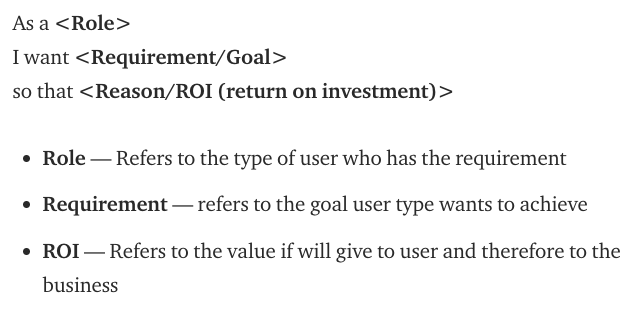
\includegraphics[width=\textwidth, frame]{UserStories_ThreeRs.png}
    \caption{3 Rs of User Stories}
    \label{fig:my_label}
\end{figure} 

For each of the user stories provided below, acceptance criteria will then follow. This aims to articulate exactly when the user story is done from product owners perspective to produce acceptance tests (SYSTANGO 2019). As this technology is targeted to assist with ethnographic data management, each user story will be from the perspective of an anthropologist.
\clearpage



    

Compatible with mobile and desktop
1. As a anthropologist, I want a data management tool that will allow me to organize, edit and store data without manipulating 

Compatible with all ethnographic data types i.e. text, photos, video, audio.
2.
Organises files with rich metadata
3.
Ability to edit files
4.
Offline function 
5.
Safe and reliable storage system
6.




\section{Acceptance Criteria}

\section{Themes in User Stories}

\section{References}
\end{document}
